\chapter{Discussion and Perspectives}
\label{chap:discussion}

{ \Large \leftwatermark{
\put(-67,-66.5){ 1 }
\put(-67,-91.5){ 2 }
\put(-67,-116.5){ 3 }
\put(-67,-141.5){ 4 }
\put(-67,-166.5){ 5 }
\put(-67,-191.5){ 6 }
\put(-67,-216.5){ 7 }
\put(-76.5,-250){\includegraphics[scale=0.8]{img/thumbindex.eps}} \put(-67,-241.5){ {\color{white} 8 }}
} \rightwatermark{
\put(350.5,-66.5){ 1 }
\put(350.5,-91.5){ 2 }
\put(350.5,-116.5){ 3 }
\put(350.5,-141.5){ 4 }
\put(350.5,-166.5){ 5 }
\put(350.5,-191.5){ 6 }
\put(350.5,-216.5){ 7 }
\put(346.5,-250){\includegraphics[scale=0.8]{img/thumbindex.eps}} \put(350.5,-241.5){ {\color{white} 8 }}
}}

\newpage

\subsubsection*{Abstract}

The enormous wealth of data generated in the life sciences presents us with incredible opportunities to improve medical genetics, but also with an equally big bioinformatics challenge to fulfill this promise.
The scope and complexity of this challenge is exacerbated by the increasing speed at which new methods, tools and data sets become available across a wide range of disciplines ranging from statistics to computer science and from model organisms to clinical validation.
In this thesis, I contributed a number of bioinformatics models, methods, and integrated systems thereof as infrastructure to enable rapid translation of these new resources into medical applications.

\subsubsection*{Introduction}

In this thesis I first developed new data management and processing models in chapter \ref{chap:xgap} and implemented these to store, integrate and visualize model organism data in chapter \ref{chap:xqtl}.
By connecting human disease phenotypes to model organisms, I showed that this approach can be used to discover new disease leads in chapter \ref{chap:wormqtl}.

I then investigated how existing methods for computational estimation of variant deleteriousness can be used to predict pathogenicity classification with high precision and recall in chapter \ref{chap:caddmmr}.
In chapter \ref{chap:gavin} I generalized this method to thousands of genes, and molecular geneticists can now use an integrated online system to classify patient DNA variants in the context of large reference data.

While new methods and data become available at ever increasing speeds, their implementation in clinical practice lags behind because of the time needed to validate and implement them into clinical practice.
To implement and validate new analysis protocols rapidly and efficiently in research and clinical practice, we need a streamlined automated pipeline for data processing, decision making, and reporting of results.
I therefore developed a software system for structured variant interpretation, currently adopted in routine diagnostics, that combines new methods and models with existing tools and knowledge databases in chapter \ref{chap:frameworkforgenomics}.

In this chapter I will consider the meaning and implications of the work presented in this thesis and look to the future potential and oncoming challenges of the field.
I first discuss in section \ref{modelsection} the successes and challenges of flexible models to capture, integrate (\ref{modelsection_integration}), share and reuse life science data (\ref{modelsection_reusable}).
I address how more people could benefit from these innovations (\ref{modelsection_spreadsheet}), and if perhaps smarter technologies are needed to get more value from complex data (\ref{modelsection_future}).

Second, I consider the challenges of method development, in which data plays a critical role in section \ref{methodsection}.
The importance of data quantity and quality is exemplified (\ref{methodsection_data}), as well as pitfalls in method benchmarking (\ref{methodsection_benchmarking}).
I highlight future ways to overcome difficulties in finding (\ref{methodsection_finding}) and running appropriate methods (\ref{methodsection_running}).

Finally, I examine how to better implement complex systems for application to medical genetics in section \ref{systemsection}.
Crucial aspects such as sharing of workflows (\ref{systemsection_reusable}) and community expertise (\ref{systemsection_community}) are discussed, and I suggest future work on multi-omics analysis (\ref{systemsection_multi}) and semantic protocols (\ref{systemsection_semantic}).
For each of the sections I will summarize key question and key points.


\sectionmark{Flexible models for life science omics data} % extra to get the top mark okay..
\section{Flexible models for life science omics data} \label{modelsection}
\sectionmark{Flexible models for life science omics data}

Life science data can be stored, managed and queried in a multitude of different ways, each with their own advantages and drawbacks.
In this section, I discuss various models and aspects involved in confronting the life science data challenge.

\subsubsection*{Key question and points of this section}

\textsl{How should data models be designed to integrate, reuse and share data from life science experiments in order to extract knowledge that benefits medical genetics?}

\begin{tcolorbox}[width=\textwidth,colframe=deeporange,colback={white},title={Key points},colbacktitle=deeporange,coltitle=black,enhanced]
  \begin{itemize}
    \item We have researched and evaluated different data integration models that make genotype-phenotype analyses more contextual and insightful (\ref{modelsection_integration}).
    \item Some applications demand greater data model flexibility, but the loss of predefined data classes presents new issues (\ref{modelsection_reusable}).
    \item Ontologies can be used to give explicit meaning back to the data, allowing methods and tools to again perform cross-set analyses (\ref{modelsection_reusable}).
    \item Managing growing quantities of life science data in spreadsheets and flat files is problematic, therefore more should be done to increase uptake of better alternatives (\ref{modelsection_spreadsheet}).
    \item Data is being shared, but without smart storage algorithms it remains difficult and time consuming to ask even basic questions (\ref{modelsection_future}).
  \end{itemize}
\end{tcolorbox}

\subsection{Integration of heterogeneous omics data} \label{modelsection_integration}

Methodological (re)use of all available life science data is difficult.
Making data suitable for reuse requires structured storage with sufficient metadata to allow retrieval and interpretation, which is troublesome and time consuming to achieve.
In addition, various storage paradigms are needed to complement traditional databases because data volumes are large and database structures often complex and highly heterogeneous\cite{Swertz_2007}, which limits interoperability and integrateability of these data.
Data covers a wide variety of phenotypic measurements including age, gender and height; answers given in questionnaires; detailed clinical observations; and large-scale molecular measurements such as DNA sequencing, gene expression, metabolomics and proteomics.
Moreover, these data may be collected from many subjects, at different timepoints, from multiple tissues, using a various wet and dry laboratory protocols.
Finally, rapid development of new profiling techniques and analysis methods requires data infrastructure to rapidly change to accommodate.

\subsubsection*{The eXtensible Genotype and Phenotype model}

We investigated how data models and supporting software systems should be (re)designed to accommodate this heterogeneity and to be effective in handling these data.
The first result was the XGAP data model developed to capture a variety of life science data that is described in chapter \ref{chap:xgap} and summarized in Box 1.

\begin{tcolorbox}[width=\textwidth,colframe=deeporange,colback={white},title={Box 1: Brief explanation of the XGAP data model},colbacktitle=white,coltitle=black,enhanced]
The innovative XGAP model facilitates integration of a wide range of data sources into one conceptual framework by enabling researchers to define observations as any combination of subjects (the thing being observed) and trait (the measurable quality).
As a result, data can be flexibly stored, eliminating the need to define the exact storage requirements for experimental data, which is impossible beforehand and moot after project completion.
For example, definitions of concepts such as 'Gene', 'Marker', 'Individual' or 'Metabolite' remain constant, but they can be used to create any dataset while the application is running.
Then gene expression data can be defined as 'Gene' $\times$ 'Individual' with a numeric value at each combination and a genotype map as 'Marker' $\times$ 'Individual' with categorical values, e.g. 'AA', 'CC', 'AC'.
After QTL analysis, the result then can be defined as 'Gene' $\times$ 'Marker' where each value indicates the statistical strength of the association between gene expression and genotype.
\end{tcolorbox}

XGAP’s flexibility is a sharp contrast to traditional applications built on relational databases that need to be taken offline for redesign when a new data modality comes in.
A life science database can now be created when a research project starts and experimental measurements plus contextual data from external providers, e.g. gene annotations or pathway definitions, added naturally as the project progresses.

We implemented XGAP into the MOLGENIS\cite{Swertz_2010a} software toolkit that generates database software infrastructure from data model and user interface specifications.
By combining the MOLGENIS software and XGAP datamodel as a foundation, we now can implement generic life science databases that can handle almost any omics/QTL data.
We published this system as xQTL workbench in chapter \ref{chap:xqtl}.
This system can handle any genotype-to-phenotype experiments and can be used as a template to create data portals for specific research areas.
We demonstrated the added value of xQTL first in \textsl{C. elegans} research\cite{Snoek_2012}, then added a translation from model organism to human disease genetics.
The resulting WormQTL\textsuperscript{HD} database\cite{van_der_Velde_2013a} is described in chapter \ref{chap:wormqtl}.
Its built-in visualization tools can be used to find clues for the molecular workings of human disease in almost 100 online-accessible datasets.

\subsubsection*{When even more flexibility is needed}

The XGAP model’s power comes from its fifty-fifty balance between static data structure (the underlying structure does not change when new data is loaded) and dynamic modeling (the structure can be easily extended and adapted and depends on the genes and phenotypes in the experimental data).
The static structure acts as a stable template that enables development of new software tools that then will work on all data loaded because the tools know what data structure to expect.
At the same time new data modalities can be rapidly accommodated using the flexible structure.

However, there are drawbacks to using (partially) static data structures.
It requires users to familiarize themselves with a data model, and limits the attributes that can be used to express information while simultaneously burdening the user with often unnecessary attributes.
An attribute is a property of the object type being described.
An object of the type 'car', for instance, can have the attributes 'brand', 'model', 'color', and 'year of construction'.
Pre-defining the attributes for data in life sciences can be very convenient for some uses, for instance if they want to automatically connecting genomic data to a genome browser.

Nevertheless, we found that more flexibility is better in some other cases.
Therefore, when we developed MOLGENIS 2.0, we created the even more flexible EMX (entity model extensible) storage model.
In MOLGENIS 2.0, the user uploading the data has full control over all aspects of the data model, meaning that tabular data can be defined at column and data type level, as well as cross-linked in any way.
This allows use of XGAP or other data models if desired.

Together with collaborators, we evaluated the models in many other online databases for various domains within life sciences\cite{Adamusiak_2012}.
Figure \ref{fig:discussion_molgenisfamily} shows the two main paths in evolution (XGAP and EMX data modeling) and a selection of currently active software applications.
These applications are powered by the MOLGENIS platform which allows flexible generation and configuration of database application.

\begin{figure*}
\centering
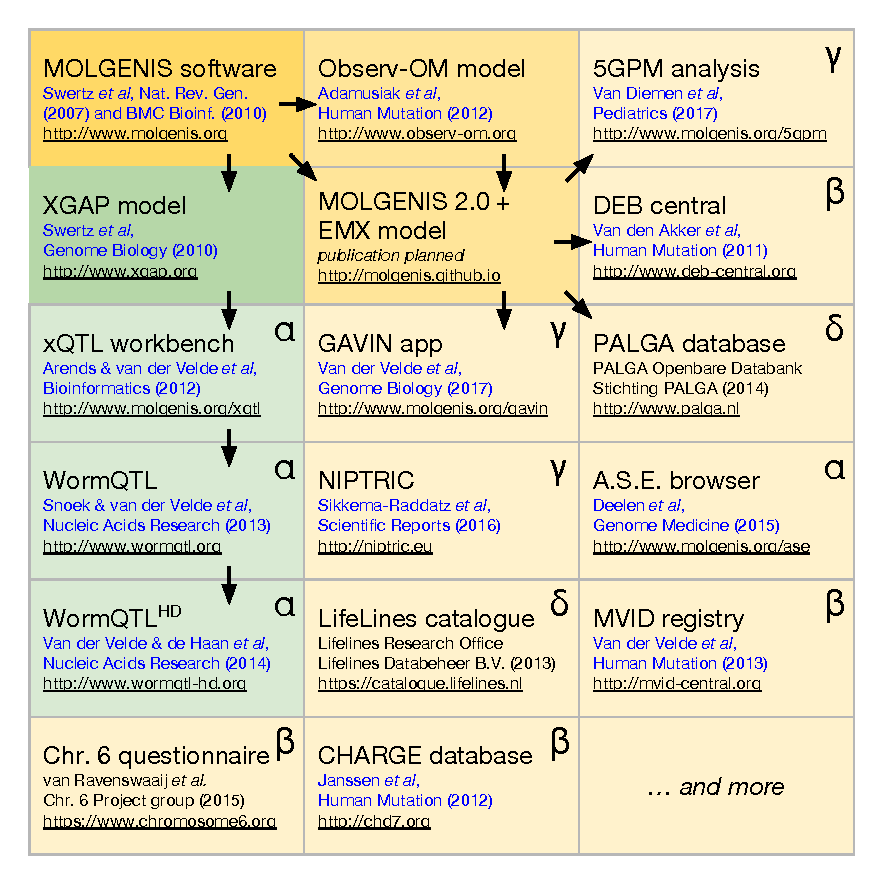
\includegraphics[scale=0.7]{img/discussion_molgenisfamily}
\caption[The MOLGENIS family of software]{The MOLGENIS family of software, data models and applications. The core software and models (top left corner) form the basis for a variety of applications, with those in green boxes directly built from the XGAP data model. The types of applications are indicated with an $\boldsymbol{\alpha}$ for research portals, $\boldsymbol{\beta}$ for patient registries, $\boldsymbol{\gamma}$ for diagnostics support, and $\boldsymbol{\delta}$ for biobank catalogues. Blue text indicates a peer-reviewed published article.}
\label{fig:discussion_molgenisfamily}
\end{figure*}

\subsection{Making omics data reusable across systems} \label{modelsection_reusable}

The most recent versions of MOLGENIS allow the user to define and import any data structure.
This is highly appreciated by users as it provides complete freedom to upload whatever data they like.
MOLGENIS uses a simple tabular format that contains both the data itself and its meta-data describing the flexible attributes with strongly-typed values.
After import, data set columns can be added, deleted or redefined if needed.
Data values can cross-reference to other datasets or rows within datasets to create a complex ad hoc data model.
Users can thus create a database perfectly tailored to their storage needs that can be re-tailored whenever those needs change.
The learning threshold of creating and managing such a database is low, and it encourages people to upload and connect any data they find relevant.
However, because the semantics of the data are now no longer explicit, this presents a new challenge.

\subsubsection*{Need standard model building blocks}

While it is now much easier to bring data together into one MOLGENIS system, the cost of this freedom is the loss the explicit meaning of the data, as compared to XGAP.
This greatly limits data re-use because data cannot be easily integrated with other datasets and analysis tools cannot be used.
In other words, for data to be reusable its semantics must be clear so humans as well as software can understand and know what to do with it. 
Users A and B may both upload a set named 'Genes', but the system does understand whether these actually refer to the same concept.
The same problem applies to any attributes within these data sets.
Perhaps they both have a 'Position' column, but one may be measured in centimorgan and the other in base pairs.
Even if the units are the same there may be crucial contextual differences, for example base pair positions that are derived from different genome builds.
This uncertainty makes it impossible to reuse tools and methods because certain necessary attributes cannot be automatically connected.

To deal with this issue, the latest MOLGENIS versions use small data models to enable implementation of standard analysis protocols without limiting the flexibility of the system.
Some data has a very predictable and often reoccurring structure. A good example is the 'genomic location’ tied to variants and other features of the DNA.
The attributes of these genomic locations are usually chromosome, position, genome build, reference and alternative base, which are automatically mapped to a micro-model and understood by the system so that tools such as the genome browser can immediately visualize the data.

\subsubsection*{Use of ontologies}

The micro-model solution is an efficient way to deal with highly predictable data.
However, most flexible data will still not be understood by the system and therefore not easily connected, integrated and analyzed.
Note that the difference between a data model and an ontology is subtle but significant, and therefore we clarify this in Box 2.

\begin{tcolorbox}[width=\textwidth,colframe=deeporange,colback={white},title={Box 2: Difference between data model and ontology},colbacktitle=white,coltitle=black,enhanced]
Ontologies can be thought of as dictionaries that define terms, with the special addition that terms can be related to each other.
Data models can be thought of as floor plans that offer explicit structure, while the definitions of the concepts used are implicit.
For example, a floor plan could specify how a living room is connected to the other rooms and show the arrangement of the furniture, whereas an ontology would define the concepts of a living room and elaborate on known types of furniture.
People who used different building plans to construct their house can use the ontology to refer to their now shared understanding of a living room, and find out if they both have a couch in it.
\end{tcolorbox}

To overcome this problem, we enable users to annotate or 'tag' their free-form data with additional meta-information that explains what the data means.
The database must contain concepts such as 'Position' measured as 'Integers' on reference build 'GRCh37' for 'Homo sapiens'.
These concepts can then be mapped on the sets, rows and columns of data sets imported.
Tools use these tags to understand the meaning of the data, which ensures that queries and tools can be reused between heterogeneous datasets.

The meta-data used to annotate data with meaning are called \textsl{ontologies}, which are common dictionaries of agreed-upon, well-defined terms and their relationships.
Building an ontology through input from an international community of domain experts ensures a shared point of reference for the clear communication of meaning.
Annotating data with ontologies offers many advantages in terms of connectivity and reasoning, but requires a significant investment of expert’s time.
To drastically lower this burden, we have developed strategies for automated matching of terms to ontologies\cite{Pang_2014} and for smart matching values to coding systems\cite{Pang_2015}.
The resulting systems allow users to harmonize data items and values in a fraction of the time it would normally cost, thereby enabling pooled data analysis for higher statistical significance.
The MOLGENIS online data platform can assist users to quickly interconnect their data via semantic annotation\cite{Pang_2015}.

\subsubsection*{Ontologies for medical genetics}

Structured ontologies also provide computational advantages.
Ontologies may be expressed as graphs of connected terms, typically a tree-shaped hierarchies where a broad root term branches out into more specific terms.
Famous ontologies used in medical genetics include ICD\footnote{http://www.who.int/classifications/icd/en} and SNOMED-CT\footnote{http://www.snomed.org} for diseases, and Gene Ontology\cite{Ashburner_2000} to describe genes.

The Human Phenotype Ontology\cite{Robinson_2010} (HPO), shown in Figure \ref{fig:discussion_hpograph}, is an ontology of particular usefulness.
HPO terms are becoming an integral component of clinical work in many medical centers, including the UMCG\cite{van_Diemen_2017}, where they are used to convey patient symptoms to the decision support software.
Symptoms can be expressed in HPO terms that may be broad or specific.
Likewise, diseases may be expressed as collections of multiple HPO terms.
Computer algorithms can accept HPO terms as inputs and take advantage of the underlying graph structure, for example, to find a known disease that best matches a set of input symptoms.
The paths between the terms are used as a distance measure, and advanced methods can even calculate semantic distance between collections of terms weighted by information content\cite{Resnik:1995:UIC:1625855.1625914}.
This clears the way for advanced tools\cite{Girdea_2013} that can guide or support a genomic diagnosis with a robust phenotypic match of patient symptoms to a known disorder for which the causal gene is known.

\begin{figure*}
\centering
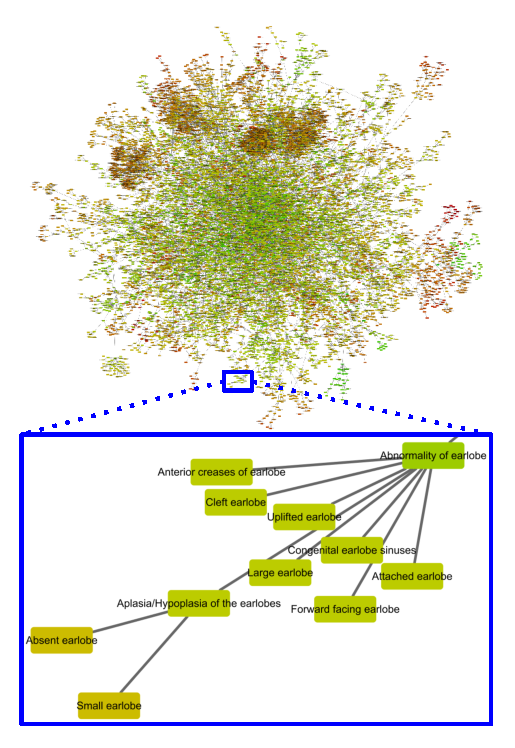
\includegraphics[scale=1.0]{img/discussion_hpograph}
\caption[Graph of the Human Phenotype Ontology]{Graph of the Human Phenotype Ontology colored by eccentricity, i.e. the distance to root node, from 0 (green) to 13 (red). The blue box shows a zoomed-in view so that labels can be read and the hierarchical structure becomes apparent. This graph has 11,044 vertices and was visualized using CytoScape (\url{http://www.cytoscape.org}) on the OBO file of HPO downloaded June 2015.}
\label{fig:discussion_hpograph}
\end{figure*}

\subsection{Spreadsheets in the era of big complex data} \label{modelsection_spreadsheet}

Many researchers, clinicians and other specialists use unsophisticated data storage methods such as spreadsheet documents.
While spreadsheets are a useful means for interacting with tabular data, they are not intended to be used as local databases for serious long-term data management.
As datasets in spreadsheets grow in size and complexity, many problems arise regarding data consistency\cite{Ziemann_2016}, corruption (e.g. the 'autocorrection' of gene names that look like dates\cite{Zeeberg_2004}), availability, versioning, performance, backups, multi-tenancy and security - nor do local spreadsheets support FAIR principles\cite{Wilkinson_2016,Wilkinson_2017} that encourage data to be Findable, Accessible, Interoperable and Reusable.

\subsubsection*{Making relational database technology accessible}

Relational database technology has developed over the many decades since its invention\cite{Codd_1970} to specialize in highly structured and consistent management of high-dimensional tabular data.
Frameworks such as MOLGENIS enable the creation of front-end web interfaces that allow relational databases to be operated in a more visual and user-friendly way.
Many software applications that were developed with the MOLGENIS framework, shown in Figure \ref{fig:discussion_molgenisfamily}, prove that this approach brings the advantages of relational databases to a variety of life science data applications that might otherwise remain hidden and vulnerable in local spreadsheets.

\subsubsection*{The challenge of big data}

Relational databases are not always an appropriate storage solution.
Huge files are currently being produced by automated data processing tools by high-throughput technologies such as whole-genome DNA sequencing.
With costs dropping and thousands of samples sequenced daily, the data is rapidly growing from terabytes to petabytes and beyond.
It would therefore be highly impractical to store each atomic value from these data in a relational structure because there is no need for this data to be query-able and a significant amount of additional disk space would be needed to index the data.

However, when thousands of individuals are profiled over many years and their data analyzed by many researchers in different projects, it is inevitable that data is lost track of.
Retrieving specific samples in that situation would involve a costly exercise in 'forensic bioinformatics'.
Projects that want make use of the data, for example a combined re-analysis of undiagnosed patients with a cardiomyopathy indication, would have to spend a significant amount of time to simply retrieve the right samples.

\subsubsection*{How to find and access large files}

A catalogue system powered by a relational database can be used to store sample metadata and file locations, along with detailed provenance of how the sample was processed and analyzed, and of the results.
Using information such as patient phenotype, tissue sampled, sequencing platform and processing software used, data of interest can be quickly found and used for analysis.

A publicly available example of such a big data catalogue is the European Genome-phenome Archive \cite{Lappalainen_2015}, which currently contains everything from raw sequencing files to genotypes called to phenotypes.
The data is organized in studies and data sets, and enriched with the provenance of samples and the technology used for analysis, e.g. "Affymetrix 500K" or "Illumina HiSeq 2000".
This allows researchers to find data appropriate for their (meta-)analysis amongst the petabytes of deposited files based on biological-, laboratory- and digital provenance.

\subsubsection*{Hybrid solutions for large data queries}

Combining relational and file-based storage can also be an effective solution.
The applications developed based on the XGAP data model, such as WormQTL\textsuperscript{HD}, employ a hybrid file-relation storage strategy.
The rows and columns link to entries in a relational database, such as Markers and Genes, which can be queried as usual, while the large data in matrix form are stored as a two-dimensionally indexed binary file.
Using the query results, data selections from the matrix based on rows and columns can be made very quickly.

The result of this hybrid design is great performance with minimal overhead and disk space requirements, but its drawback is that sorting and filtering operations on non-indexed matrix values are slow.
These queries are however not important for the main use-cases of this database, so the overall solution worked out very well.
This shows that no solution is perfect, but the success of a system does depend on the storage strategy chosen.

\subsubsection*{Basic data management training for all life science researchers}

We have shown many different models, methods and tools to manage life science data, from relational databases with static and dynamic models to relational-file hybrids and file-catalogue systems.
There is no single “best” solution: each of these approaches represents a valid solution for different storage and query requirements, which just underscores the need for flexible systems that can adapt to future data structure needs and switch to storage backends that scale to bigger data volumes when required.

However, the average researcher has little interest in the technical background of these solutions and simply wants a system that capable of serious data management that is still as comfortable to use as a spreadsheet program.
Making the transition requires an investment of time and energy that is sometimes not well understood and/or seen as too burdensome.
Parties that offer data management solutions may have a responsibility to underscore the importance of helping people to use better data management.
We suggest number of actions to facilitate the uptake of better data management tools in Box 3.

\begin{tcolorbox}[width=\textwidth,colframe=deeporange,colback={white},title={Box 3: Actions towards uptake of better data management tools},colbacktitle=white,coltitle=black,enhanced]
\begin{enumerate}
  \item Raising awareness of the dangers and limitations of using spreadsheets and other inappropriate solutions for data management. This is also the mission of the European Spreadsheet Risks Interest Group\footnote{\url{www.eusprig.org}}.
  \item Increasing the visibility of alternatives by shifting the focus of publications, workshops and presentations from specific applications back towards the importance of underlying technologies such as the MOLGENIS platform.
  \item Making demonstrations publicly usable in an unrestricted but private way to those who are interested. Subsequently, non-technical users should be able to immediately create secure instances in the cloud suitable for sensitive data. For technical users, it should be simply to run the software on their own servers.
  \item To keep initial interest alive, the thresholds of starting to use these applications must be as low as possible. Data management should be user-friendly overall, but it is critical that systems be fault-tolerant so aspiring users are not punished by having to fix many small mistakes when importing their data. Data should also be importable in the simplest of formats and even via direct entry, i.e. similar to using spreadsheet software.
  \item Those exploring the system more deeply must experience clear benefits and advantages. For instance, a user-friendly data explorer should offer powerful options to find, filter, sort and plot the data, as well as guarantee consistency, security and easy sharing with colleagues.
\end{enumerate}
\end{tcolorbox}

\subsection{Future perspectives of sharing life science data} \label{modelsection_future}

The life science and molecular medicine community is gathering, using and sharing tremendous amounts of data. 
Popular published data resources include the Genome of the Netherlands\cite{Francioli_2014}, Ar\-ray\-Ex\-press\cite{Rustici_2012}, 1000 Ge\-no\-mes Pro\-ject\cite{Auton_2015}, Va\-ri\-Bench\cite{Nair_2012}, Blood eQTL brow\-ser\cite{Westra_2013}, database of Geno\-types and Pheno\-types\cite{Mailman_2007}, Clin\-Var\cite{Landrum_2013}, Exome Aggregation Consortium\cite{Lek_2016}, genome Aggregation Database\footnote{\url{http://gnomad.broadinstitute.org/}}, RNA-seq ASE brow\-ser\cite{Deelen_2015}, Eu\-ro\-pe\-an Nu\-cleo\-tide Ar\-chive\cite{Leinonen_2010} and Ge\-no\-type-Tis\-sue Ex\-pres\-sion\cite{Lonsdale_2013}.
Making these data open and freely available generates a higher number of citations and increases their overall prestige, which should clearly outweigh any benefits of 'keeping data to yourself'.
Further, an increasing number of (often high-impact) scientific journals and public funding bodies require any data in publications to be openly accessible (the ideal) or at least available on request.
In fact, it is now possible to publish data as standalone resources, for example in journals such as \textsl{Scientific Data} or initiatives such as \textsl{DataCite}.
The field of genetics is indeed a frontrunner "whose sharing of data markedly accelerated progress"\cite{Rosenbaum_2017} compared to fields such as clinical trials.

Indeed, we ourselves opened up dozens of research datasets and results in the WormQTL\textsuperscript{HD} database, free to download without restrictions for anyone interested .
Conversely, the methods presented in chapter \ref{chap:caddmmr}, the CADD scores for MMR genes, and GAVIN in chapter \ref{chap:gavin}, could not have been developed without free and publicly available datasets.

\subsubsection*{New query options are needed for humans and computers}

While incredible datasets are currently being generated, the development of software tools to interact with these data seems to be lagging behind.
Even relatively simple questions such as "How many variants at exon 10 of the TTN gene are exclusive for individuals of Asian descent?" cannot easily be asked because
(i) most resources do not have an adequate query interface,
(ii) query interfaces do not understand or support the question, and
(iii) there is no cross-database "Google-like" interface to query all potential sources at once.
We could fulfill the promise of systems biology research to create understanding of life in a bigger context by being able to routinely run deep complex queries across our complete knowledge of organisms, phenotypes, populations, tissues, metabolites, genetics, drugs, and so on.

\subsubsection*{Ontologies, semantics and FAIR solutions}

This situation can be improved by increased usage of ontologies.
Data may be expressed as \textsl{nanopublications}, i.e. predicated relationships between two ontological concepts with provenance attached.
For example, we can express knowledge into formal terms as follows:
the CENPJ gene (\url{http://bio2rdf.org/geneid:55835}) has a statistical association (\url{http://semanticscience.org/resource/SIO_000765.rdf}) to Seckel Syndrome (\url{http://bio2rdf.org/omim:210600}) of 0.00006562\footnote{Example taken from: \url{http://nanopub.org/wordpress/?page_id=57}.}.
Data can be freely reasoned upon once expressed in a formal and semantic way, as demonstrated in case studies\cite{Mina2015}.
The underlying RDF\cite{RDF-PRIMER} (Resource Description Framework, a way to semantically describe data) and SPARQL\cite{Prudhommeaux08} (Simple Protocol And RDF Query Language, a way to question semantic data) technologies are supported by the Linked Data initiative\footnote{\url{http://linkeddata.org}}, which aims to connect structured data on the internet, essentially turning it into a giant database.
It has also been shown that semantic queries can indeed be used for both generating and evaluating hypotheses\cite{Mina2015,Callahan_2011}, and assist in genomic variant prioritization\cite{Boudellioua_2017}.

Although some large organizations offer proper RDF access\cite{Jupp_2014} and third-party tools are written for others\cite{Anguita_2013}, this technology is hardly a cornerstone of modern life science databases.
It can be quite labor-intensive to completely ontologize a database for RDF support and setting up an active SPARQL endpoint.
The FAIR principles\cite{Wilkinson_2016,Wilkinson_2017} offer an alternative with much lower barriers.
FAIR is essentially a checklist to guide technical solutions and their practical applications to make data more Findable, Accessible, Interoperable and Reusable.
When fully realized, every aspect of data would be annotated with semantic metadata for complete and seamless reusability.
The MOLGENIS/XGAP work presented in this thesis are in that sense FAIR systems, created before that term was coined.

Given the challenges of building and using datamodel based storage systems this is not always attainable.
However, the guidelines can be followed to make data discoverable and searchable in simpler ways, which is always better than not at all.
An example of an easy and lightweight solution to make resources better findable by search engines is to add Bioschemas\footnote{http://bioschemas.org} semantic markup.
Other databases, platforms and initiatives such as Dataverse\cite{Crosas_2016}, FAIRDOM\cite{Wolstencroft_2016}, ISA\cite{Sansone_2012} and Open PHACTS\cite{Harland_2012} showcase other implementations and applications that are based on FAIR principles.

\subsubsection*{Federated queries require an attitude shift}

In addition to new data models and tools, I think we also need to change our attitude towards sharing and integration of query results.
Data sizes are rapidly increasing and much data is privacy sensitive, factors that make it unlikely that all data relevant to a given study will always be available in one place.
New data analysis paradigms are being developed to address this, of which so-called 'federated analysis', is a prominent example\cite{Gaye_2014,Jochems_2016}.
A federated query is executed on multiple independent locations, after which the partial results are combined into the final answer.
The nature of federated queries on multiple external sources is that the answer of today may be different from the answer of tomorrow.
This can be seen as a limitation, but can also be considered an opportunity where researchers and even clinicians always have access to the latest and greatest knowledge.
Instead of statically versioning complete data sources as a reference point, we must consider making our data dynamic and compensate for perceived uncertainties by storing the questions together with detailed data and source provenance used to compile the answer.

\subsubsection*{Legal aspects of data sharing}

Until here I have discussed life science data sharing from a mostly technical point of view.
It is however important to realize that even the most brilliant solution is pointless if the law precludes sharing and reuse of data.

Currently, data and privacy laws are being revised in light of social media and the other 'tech giants' who are gathering massive amounts of sensitive user data.
While citizens will benefit from better privacy protection, the same rules impede cohort-based biomedical research by requiring participant re-consent every time the data is used\cite{natedit_2015}.

While scientific representatives are gaining concessions on behalf of research, their legal struggle is not yet over.
Establishing fitting international legislation with many stakeholders across cultural barriers is difficult, as is the practical implementation of new rules by the science community\cite{Litton_2017}.

Perhaps by overcoming these legal growing pains, current hindrances for sharing and reusing biomedical data across the international community can be lifted, benefitting researchers and ultimately patients.


\sectionmark{Developing comput. methods for med. genetics} % extra to get the top mark okay..
\section{Developing computational methods for medical genetics} \label{methodsection}
\sectionmark{Developing comput. methods for med. genetics}

So far I have investigated models to store, access, share and query data measured and calculated in life science experiments to gain new insights.
In this section, I discuss challenges and solutions in the development and, more importantly, validation of new methods and algorithms to make most use of all these new data.

\subsubsection*{Key question and points of this section}

\textsl{How can we develop, characterize, find, share and reuse high-quality computational methods as part of new analysis protocols for medical genetics?}

\begin{tcolorbox}[width=\textwidth,colframe=deeporange,colback={white},title={Key points},colbacktitle=deeporange,coltitle=black,enhanced]
  \begin{itemize}
    \item The performance of newly developed methods depends on both the quality and quantity of available data. We must therefore cherish and share gold standard data (\ref{methodsection_data}).
    \item Reporting the strengths and weaknesses of a method in greater detail next to the overall performance is crucial for choosing the right analysis method to obtain better research or diagnostic results (\ref{methodsection_benchmarking}).
    \item We need detailed catalogs where researchers and clinicians can seamlessly find these assessments (\ref{methodsection_finding}) and run the right tool for their data and hypothesis (\ref{methodsection_running}).
  \end{itemize}
\end{tcolorbox}

\subsection{Method dependance on high quality data} \label{methodsection_data}

The genome of an average person contains around 5,000 unique mu\-ta\-tions\cite{Walter_2015}.
To establish a molecular diagnosis in an individual with a suspected genetic problem, we need to quickly reduce the number of candidate variants from thousands to just a few.
Computer algorithms can predict how harmful mutations are, but the strength of these predictions depends on the availability and quality of reference data.
These gold standard reference data are used to develop new algorithms, which are then validated on a similar but independent data set.

In this section we show that both quality and quantity of data have an effect on the predictive power of new methods.
Sharing data is therefore crucial for developing the best possible tools, resulting in more accurate prioritization and less time spent on manual assessment.
We therefore must engage in active international collaboration to set up systems for joint interpretation and open sharing of variants.
To accomplish this goal we need to overcome technical and legal barriers, but it is also a social challenge, as labs can be distrustful of other labs that operate under different guidelines or less stringent quality standards.

\subsubsection*{CADD and GAVIN}

CADD scores\cite{Kircher_2014} are a promising method to estimate pathogenicity of any mutation in the genome.
We calibrated CADD in silico pathogenicity estimates to help classification of mismatch repair gene variants in chapter \ref{chap:caddmmr}.
We used variants assessed by an international committee of domain experts to establish the relationship between CADD scores and classification outcome.
This was very successful, and this success was helped by the outstanding quality of the reference data set we used.
Re-application of this model to the original data showed only a few discrepancies, and they could all be explained in favor of the original human expert classification.

This work was followed up in chapter \ref{chap:gavin} where we present the GAVIN variant classification tool for $>$3,000 clinical genes.
Interestingly, we found that CADD-based predictions work better for some genes than for others.
This may be explained by currently unknown biological differences that are not captured in the in silico pathogenicity estimates we used, however a simpler explanation is that the expert variant classifications were of lower quality for certain genes, and those mistakes distorted the calibration. 
We have already shown that for genes with enough training data we get better classification accuracy than we do for genes for which scarce data is available, but here we can investigate the relationship of both quantity and quality of gold-standard data with calibration success in more detail.

\subsubsection*{Association of p-value with variant quantity and quality}

The GAVIN gene calibrations include a Mann-Whitney U test p-value for the tested significance of the CADD score difference between pathogenic and matching benign variants.
The lower a p-value for a gene, the more reliable and useful the gene calibration becomes for automated variant classification.
These gene calibration p-values can be plotted against the number of expert-assessed pathogenic variants available per gene.
For this we used the ClinVar variant\_summary.txt file of 1/12/2016, downloaded from \url{ftp://ftp.ncbi.nlm.nih.gov/pub/clinvar}).
The result can be seen in Figure \ref{fig:discussion_nrofvariantsvspvalue}.
Indeed, a simple log-linear model shows a trend in which gene p-values become more significant as the quantity of available variant classifications increases.

\begin{figure*}
\centering
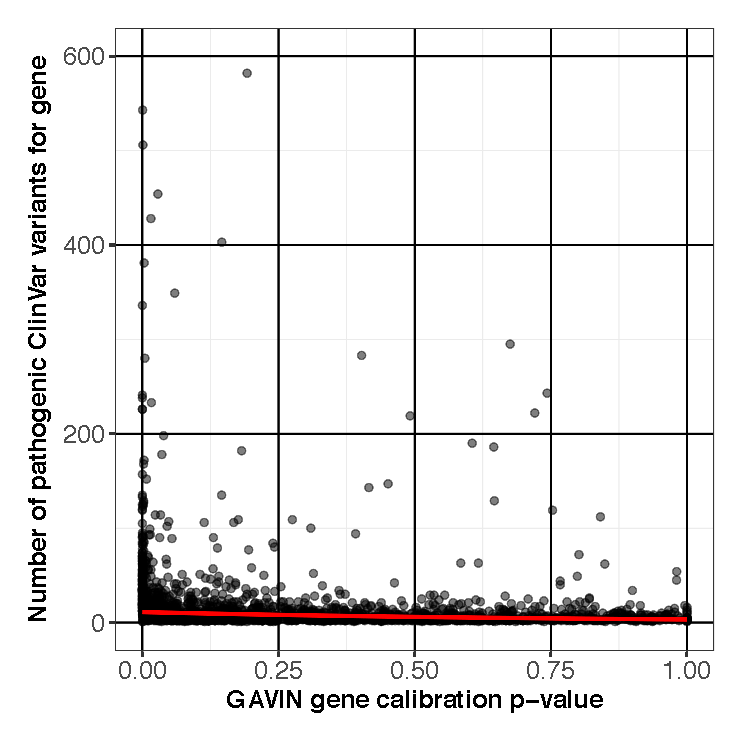
\includegraphics[scale=0.8]{img/discussion_nrofvariantsvspvalue}
\caption[Relation between calibration and number variants]{Relation between calibration success and the number of pathogenic variants available for that gene. Log\textsubscript{10} linear regression (shown in red) resulted in \textsl{R\textsuperscript{2}} = 0.11 and \textsl{p}-value = 7.28e-57.}
\label{fig:discussion_nrofvariantsvspvalue}
\end{figure*}

To measure variant interpretation quality, we can use the review status of ClinVar variants.
The review status shows the amount of supporting evidence for the clinical significance (i.e. classification) of a variant.
The text values also correspond to a 'star' rating from 0 to 4 (see Table \ref{table:reviewstatustostars} on how the terms are mapped), which can be used quantitatively.
We can take the mean of this rating per gene as a measure for interpretation quality.
When plotted against the gene calibration p-values (Figure \ref{fig:discussion_reviewstatusvspvalue}), there is a trend in which gene p-values become more significant as the quality of variant classifications increases.

\begin{table}
\begin{tabulary}{\linewidth}{LL}
  ClinVar review status & 'Star' rating \\
  \hline
  No assertion provided & 0 \\
  No assertion criteria provided & 0 \\
  No assertion for the individual variant & 0 \\
  Criteria provided, single submitter & 1 \\
  Criteria provided, conflicting interpretations & 1 \\
  Criteria provided, multiple submitters, no conflicts & 2 \\
  Reviewed by expert panel & 3 \\
  Practice guideline & 4 \\
  \hline
\end{tabulary}
\caption[ClinVar review status and star rating]{ClinVar review status and how this translates to a numeric range, i.e. the corresponding review status 'star' rating. See \url{https://www.ncbi.nlm.nih.gov/clinvar/docs/variation_report}}
\label{table:reviewstatustostars}
\end{table}

Both trends seem to indicate that both quality and quantity of data are important when developing new methods based on previous observations to help us interpret unprecedented amounts of new data.
Therefore, we need to treasure the results of expert interpretation and analysis that has been made freely available, but at the same time put more effort into integration and 'FAIR-ification' of the many sources to achieve the best and most complete reference set possible\cite{Brookes_2015} for human health and disease.
This need will become more pressing as the amount of data grows quickly, and the upcoming demand for powerful methods that can deal with new diagnostic data modalities such as non-coding DNA, RNA-sequencing, metabolomics and epigenomics.

\begin{figure*}
\centering
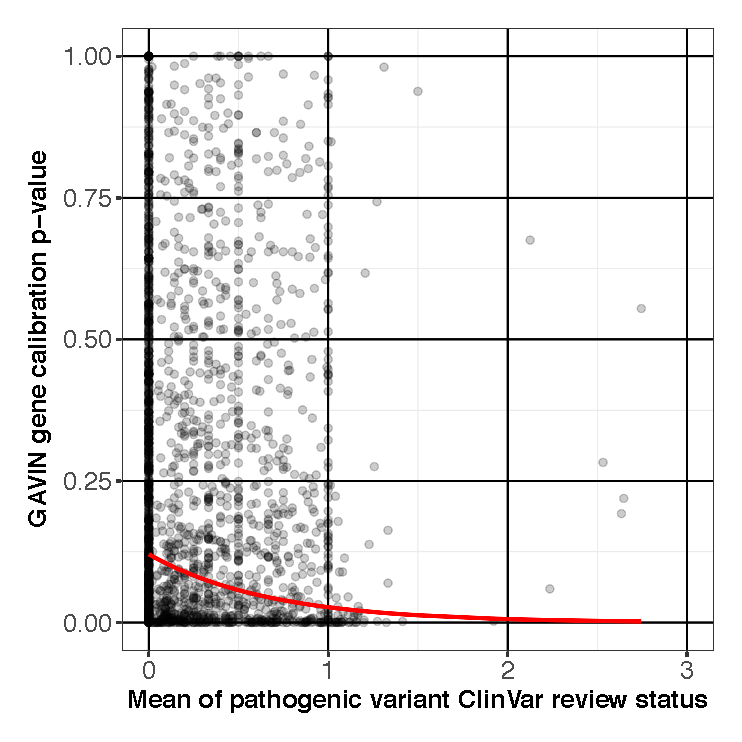
\includegraphics[scale=0.8]{img/discussion_reviewstatusvspvalue}
\caption[Relation between calibration and review quality]{Relation between calibration success and the average review quality for that gene. Log\textsubscript{10} linear regression (shown in red) resulted in \textsl{R\textsuperscript{2}} = 0.03 and \textsl{p}-value = 5.95e-16.}
\label{fig:discussion_reviewstatusvspvalue}
\end{figure*}

\subsection{Benchmarking and characterization of methods} \label{methodsection_benchmarking}

While overall performance is a good metric to judge a method's ability to screen a large set non-specific data, for specific data we should characterize a method in more detail.
In order for methods to become trusted and accepted by users such as clinical geneticists, they must know how well a method behaves and if it succeeds in situations they are familiar with.

A good example is our analysis of CADD scores for MMR genes in chapter \ref{chap:caddmmr}, where we delved into the strengths and limitations of this method when applied to four specific genes.
Developing a new method as a black box, with just an overall reported accuracy (e.g. "93\% AUC") may lead to some skepticism from those using the methods in practice, especially since most methods claim to be the best.
Instead we should characterize and report the strengths and limitations of a method, and communicate clearly that method performance may depend on the context it is used in.

The GAVIN gene calibrations in chapter \ref{chap:gavin} are reported in categories where 'C1' indicates a high degree of separation between pathogenic and benign variants and 'C4' indicates a poor separation.
These indications show that classifications in certain genes are better than in others, even though the overall performance is high.
Reporting the performance on a gene-level helps researchers or clinicians to select the best method for their specific question.

It must be noted that GAVIN reports no formal information beyond the gene level, and that there are indeed instances where more sophisticated definitions are beneficial.
We will now show three examples of genes where in-depth characterization is indeed relevant and how this may lead to tailored or optimized usage.

\subsubsection*{Examples of in-depth gene characterization}

The gene SCN5A, which encodes sodium channel type V and is associated to dominant atrial fibrillation/long QT syndrome, is an example where there is a high degree of separation and an overall great calibration.
However, notice the cluster of pathogenic variants around location 38655000 that dips below the calibration line in Figure \ref{fig:discussion_scn5a}.
This gene-specific model may be improved by local correction of the threshold for this effect.

\begin{sidewaysfigure*}
\centering
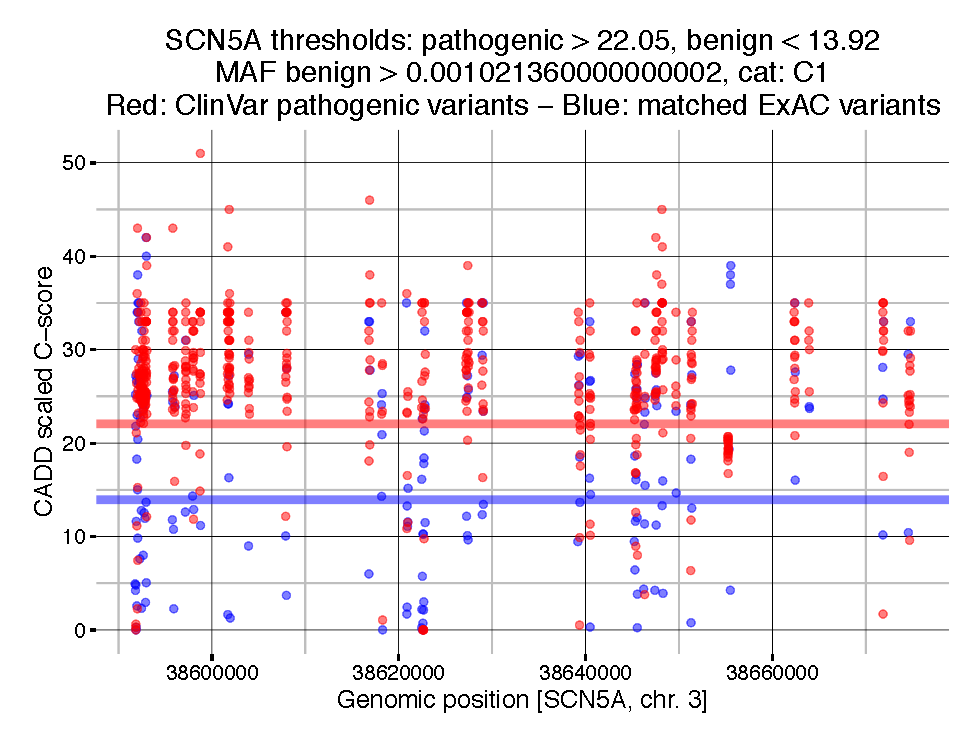
\includegraphics[scale=0.8]{img/discussion_scn5a}
\caption{GAVIN (r0.3) calibration plot for SCN5A.}
\label{fig:discussion_scn5a}
\end{sidewaysfigure*}

In the gene TTN, which encodes the protein titin and is associated to dominant cardiomyopathy, this effect is far more pronounced with a massive cluster of extremely high score pathogenic variants in the first 30\% of the gene.
See Figure \ref{fig:discussion_ttn}.
The remaining pathogenic variants appear to be distributed amongst the benign variants, making a potential two-part model perhaps complicated, but much more powerful.

\begin{sidewaysfigure*}
\centering
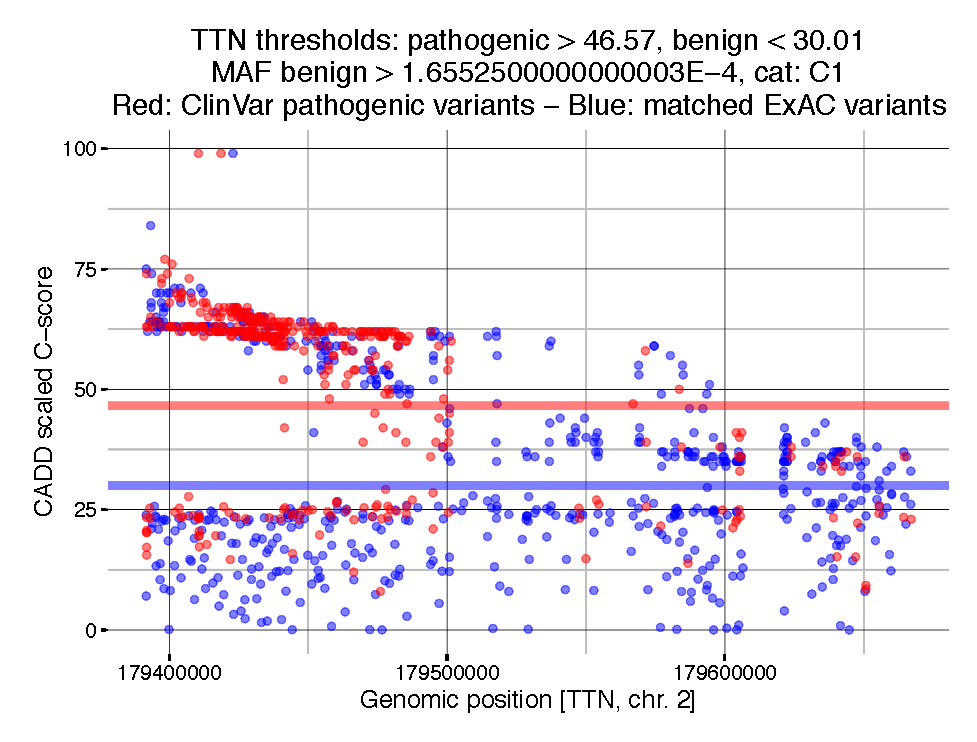
\includegraphics[scale=0.8]{img/discussion_ttn}
\caption{GAVIN (r0.3) calibration plot for TTN.}
\label{fig:discussion_ttn}
\end{sidewaysfigure*}

An example where the method offers little predictive value is the gene F11, which is associated to blood coagulation factor XI deficiency and is often recessive.
The benign variants that remain after the filtering stage of GAVIN calibration are distributed uniformly across the pathogenic variants as can be seen in Figure \ref{fig:discussion_f11}.
A simple explanation of this might be that this is a relatively mild and recessive disorder under apparently little selective pressure, which is consistent with it being relatively common among Ashkenazi Jews\cite{Seligsohn1223}.
What this example shows is that some pathogenic variants seem to be quite tolerated in the general population, blurring the line between 'benign' and 'pathogenic', therefore deleteriousness may be hard to estimate computationally.

\begin{sidewaysfigure*}
\centering
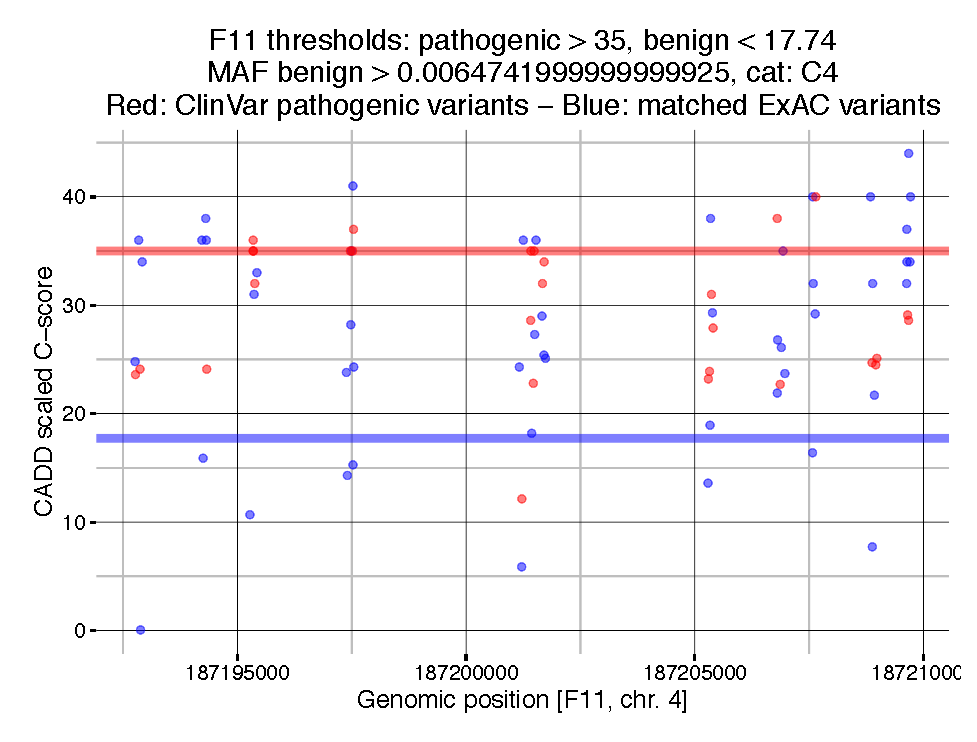
\includegraphics[scale=0.8]{img/discussion_f11}
\caption{GAVIN (r0.3) calibration plot for F11.}
\label{fig:discussion_f11}
\end{sidewaysfigure*}

\subsubsection*{Implications of method characterization}

These examples illustrate the advantages and limitations of a gene-based variant classification method.
This characterization will also apply to other data modalities including gene expression and metabolites and across different conditions such as tissue type, cell types, age, and ethnicity.
If we want to develop methods that bring these new types of information to the clinic, we must have transparent and widely accepted validation procedures and be clear on what methods can and cannot do, to prevent disappointed users.
The context for which the tool has been developed, as well as its strengths and weaknesses, should be made clear even on a gene-specific level because this knowledge may be more important than the overall performance of the method.
I think it may be worthwhile to create a truly standardized benchmark to assess and compare the methods currently available as well as those that will be developed in the future.

\subsection{Finding appropriate methods in repositories} \label{methodsection_finding}

The sequencing of thousands of patients and healthy individuals worldwide, combined with the sequenced genomes from thousands of different organisms, has spurred the development of countless methods that predict variant pathogenicity, mostly based on estimated protein conservation.
Examples of various scope and quality include: SIFT\cite{Kumar_2009}, Po\-ly\-Phen2\cite{Adzhubei_2010}, PRO\-VEAN\cite{Choi_2012}, PON-P2\cite{Niroula_2015}, Mu\-ta\-tion\-As\-ses\-sor\cite{Reva_2011}, FATH\-MM-MKL\cite{Shihab_2015}, Con\-del\cite{Gonz_lez_P_rez_2011}, Phy\-lo\-P\cite{Pollard_2009}, UMD\--Pre\-dic\-tor\cite{Fr_d_ric_2009}, Gran\-tham\cite{Grantham_1974}, ENT\-PRISE\cite{Zhou_2016}, PHAST\cite{Zhou_2011}, Fit\-Cons\cite{Gulko_2015}, Mut-\\Pred\cite{Li_2009}, EI\-GEN\cite{Ionita_Laza_2016}, GERP++\cite{Davydov_2010}, VAAST\cite{Kennedy_2014}, Align\-GV\-GD\cite{Tavtigian_2005}, MAPP\cite{Tavtigian_2008}, Mu\-ta\-tion\-Tas\-ter\cite{Schwarz_2014}, VI\-PUR\cite{Baugh_2015}, RE\-VEL\cite{Ioannidis_2016}, CADD\cite{Kircher_2014}, LIN\-SIGHT\cite{Huang_2017}, FATHMM-XF\cite{Rogers_2017} and GA\-VIN\cite{van_der_Velde_2017}.
These tools are being improved and invented in a fast competitive cycle as more benchmark data becomes available every day due to the interpretation help of the previous tool generation.

Similarly, thousands of methods for all kinds of applications, analyses and data types have been created across all branches of life sciences.
However, for a researcher at the beginning of a project, the question remains: How do I find the best methods for my analysis question? 

Search engines to find methods such as OmicsTools\footnote{\url{https://omictools.com}, currently hosting $>$17,000 entries} have emerged to let users find methods of interest.
In OmicsTools, users can browse methods via search box or by drilling down in categories.
Users can also post reviews and rating to let others know how well they liked the tool.
OmicsTools does not, however, allow more fine-grained searches that can:
\begin{itemize}
  \item Find tools that are applicable to your data, e.g. quickly finding which analyses can be run on your data.
  \item Find tools that produce a specific type of output, e.g. if you are interested in a specific type of output such as gene annotations and want to list any tools that can provide this.
  \item Find tools that perform a specific role, e.g. when you want to benchmark your method to any tool that performs the same function regardless of input or output.
\end{itemize}

The Elixir Tools and Data Services Registry\cite{Ison_2015}\footnote{\url{https://bio.tools}} tries to solve this issue by attaching EDAM\cite{Ison_2013} ontology terms to the function, topic, inputs and outputs of each method.
Tags, documentation, publication, links and contact information are also provided, together forming a comprehensive and highly structured collection of bioinformatics software.

These solutions are a step in the right direction, but they do not address two major needs: (i) providing a standardized and detailed benchmark of tool performance (as discussed earlier) and (ii) helping the user to install and run the tool of interest.
Therefore, there is still a duty for the bioinformatics community to create a central repository of documented, tested and runnable bioinformatics tools, in the same spirit as e.g. the CRAN repository for R packages.

\subsection{Integrating and running methods for evaluation} \label{methodsection_running}

Evaluating new tools in practice requires a quick process of installation and running.
This is difficult for methods that can not be offered as web services due to transfer limitations or patient confidentiality, and must therefore be compiled or installed locally and subsequently integrated into an analysis protocol.
BioContainers\cite{da_Veiga_Leprevost_2017} solve some of these issues by wrapping individual tools in container engines (Docker and rkt).
The tools retain their identity while being easier to run cross-platform.

The fast uptake of methods is much easier and quicker when they are wrapped or created for an existing workflow engine.
MOLGENIS Compute protocols\footnote{https://github.com/molgenis/NGS\_DNA/tree/master/protocols} and Galaxy tools\footnote{https://toolshed.g2.bx.psu.edu/} are method libraries for their respective workflow engines that come with descriptions and technical definitions for their inputs and outputs.
Taverna\cite{Wolstencroft_2013} workflows can be constructed and shared on My\-Ex\-pe\-ri\-ment\cite{Goble_2010}\footnote{\url{https://www.myexperiment.org}} using components\footnote{http://www.taverna.org.uk/documentation/taverna-2-x/components/} that can be linked to ontological terms for their input, output and activity.

However, there does not seem to be much emphasis on semantic description of workflow engine components in general.
Taverna components can only be published within the definitions of conventional workflows, making them difficult to find.
Methods wrapped for Compute and Galaxy do not explicitly link to ontologies at all.

These limitations were recognized and addressed by the BioMOBY method and its successor SADI\cite{Wilkinson_2010,Withers_2010}.
SADI is a method to set up discoverable semantic web services from regular databases, and has a Taverna plugin to access these services.
Unfortunately this project has been silent since 2014 and the plugin is only available for the outdated Taverna versions 2.1.2 and 2.2 (current version is 2.5).

Taken together, we find many great initiatives that collect, describe and offer methods focused on different aspects.
Unfortunately there is currently no standardized complete solution that allows a user to seamlessly discover, run and integrate methods into their analysis workflows.

There is a growing focus on the FAIR principles to make data reusable, but the exact same principles should also apply to tools.
I think we should treat tools as 'runnable data', meaning that they must be as easy to find, understand and use as data itself.
In practice, the most popular tools are simply those that are easily runnable, and these are not necessarily the best at what they do.
By applying FAIR principles to remove some of the barriers to use, we could exchange and adopt more appropriate tools to the tasks at hand.


\sectionmark{Towards better systems for (gen)omic medicine} % extra to get the top mark okay..
\section{Towards better systems for (gen)omic medicine} \label{systemsection}
\sectionmark{Towards better systems for (gen)omic medicine}

Thus far I have discussed models to store, manage, share and query life science data in smarter and better ways.
I then looked at the challenges of developing, characterizing and discovering new methods.
In this section I focus on challenges and solutions in translating new data and methods to health research and patient care.
Note that the terminology used in this section can be confusing and is therefore explained in Box 4.

\begin{tcolorbox}[width=\textwidth,colframe=deeporange,colback={white},title={Box 4: Clarification of terminology},colbacktitle=white,coltitle=black,enhanced]
In a typical data processing scenario, multiple tools or methods are connected in a workflow, also called a pipeline, which is a sequence of events through which data is processed to reach a final state.
A workflow that has been formalized into an official procedure that is agreed upon and usually versioned is what we call a protocol.
The steps within a protocol can be implemented using different tools for each step, where tools are implementations of methods.
Lastly, a system is a piece of software that executes workflows or protocols and manages their inputs, tools, outputs, provenance and other related data.
Some of these terms are used interchangeably when context allows it, for instance, workflow and protocol are in often in practice not that different.
\end{tcolorbox}

\subsubsection*{Key question and points of this section}

\textsl{How can we bring data and methods together in flexible and scalable multi-omics analysis protocols and software systems for future patient care?}

\begin{tcolorbox}[width=\textwidth,colframe=deeporange,colback={white},title={Key points},colbacktitle=deeporange,coltitle=black,enhanced]
  \begin{itemize}
    \item There is a plethora of academic and commercial software for DNA analysis, but their protocols and data sources are quite static (\ref{systemsection_reusable}).
    \item Workflow engines offer greater flexibility for data processing and are far more future-proof, but the use of a common language must be encouraged (\ref{systemsection_reusable}).
    \item Protocol implementations of best practice guidelines should be a community effort including common automated benchmarking and validation (\ref{systemsection_community}).
    \item As multi-omics analysis starts to complement routine DNA diagnostics, experts from the disciplines involved will need to contribute their best practices in a combined approach (\ref{systemsection_multi}).
    \item To keep multi-omics diagnostic protocols up-to-date, we should consider using smart workflows with abstract step definitions that automatically select the best or most appropriate tools for the job (\ref{systemsection_semantic}).
  \end{itemize}
\end{tcolorbox}

\subsection{Reusable and flexible DNA analysis workflows} \label{systemsection_reusable}

Since DNA sequencing has become popular, plenty of integrated systems have been developed that cover complete genome analysis workflows.
Commercial examples include products such as Alamut\footnote{\url{http://www.interactive-biosoftware.com}}, SeqPilot\footnote{\url{http://www.jsi-medisys.de}}, Omicia\footnote{\url{https://www.omicia.com}}, Sophia\footnote{\url{http://www.sophiagenetics.com}}, NextBio\footnote{\url{https://www.nextbio.com}}, Cartagenia\footnote{\url{http://www.agilent.com}}, MedGenome\footnote{\url{https://www.medgenome.com}}, VariantStudio\footnote{\url{http://variantstudio.software.illumina.com}}, GoldenHelix\footnote{\url{http://goldenhelix.com/}}, Ingenuity\footnote{\url{https://www.qiagenbioinformatics.com}}, Bina\footnote{\url{http://www.bina.com}}, Enlis\footnote{\url{https://www.enlis.com}} and Genomatix\footnote{\url{https://www.genomatix.de}}.
Alternatives developed in academia, often free to use, include SpeedSeq\cite{Chiang_2015}, GE\-MI\-NI\cite{Paila_2013}, In\-ter\-Var\cite{Li_2017}, Ge\-no\-mi\-ser\cite{Smedley_2016}, eXtasy\cite{Sifrim_2013}, VAAST\cite{Kennedy_2014}, SG-AD\-VI\-SER\cite{Pham_2015}, IM\-PACT, Seq\-Mule\cite{Guo_2015}, TAPER™\\\cite{Glanzmann_2016}, Clin\-Lab\-Ge\-ne\-ti\-cist\cite{Wang_2015}, WGSA\cite{Liu_2015} and wAN\-NO\-VAR\cite{Chang_2012}.
These systems are quite specific for the types of data and questions they can handle.
Either they offer a built-in analysis or they allow the user to select which of the preconfigured data and filters should be used.
While these products may perform their function well, the lack of freedom can be a serious restriction.
The GAVIN+ tool presented in chapter \ref{chap:frameworkforgenomics} is guilty of the same, although it is part of a bigger genome interpretation framework with options for customization and tool replacement.

With many new sources of data, knowledge and tools are quickly becoming available, typical genomics analysis software cannot keep up with the demand for the latest and greatest developments, let alone support integrating completely new data modalities such as RNA-seq, metabolomics and epigenetics.
Switching to different software or adopting multiple tools to use the best features of each is time consuming and expensive, while using an incomplete solution means missing out on the best research results or diagnostic answers.

\subsubsection*{Workflow engines, a better way?}

Workflow engines offer part of the solution to these issues.
They are a type of software not tied to specific data types or analysis protocols, but instead offering the flexibility of letting users define and share their own analyses.
Examples include Ga\-la\-xy\cite{Goecks_2010}, Ta\-ver\-na\cite{Wolstencroft_2013}, An\-du\-ril\cite{Ovaska_2010}, UGENE\cite{Okonechnikov_2012}, Gene\-Pat\-tern\cite{Reich_2006}, Vis\-Trails\cite{Bavoil_2005}, Ar\-va\-dos\footnote{\url{https://arvados.org}}, AWE, Toil, Ra\-bix and MOL\-GEN\-IS Compute\cite{Byelas_2013}.
In these software the user has full control and freedom over analysis steps such as choosing which tool and data dependencies are used. 
A user can, for instance, choose GATK\cite{Van_der_Auwera_2013} for genotype calling then subsequently choose PLI\-NK\cite{Purcell_2007} for association analysis.
The flexibility originates from using simple tool input/output structures that are typically file based.
This agnostic approach to handling data makes it easy to hook up new tools and file formats.
Due of their adaptability these solutions are more future-proof than software shipped with built-in analyses.
However, the graphical user interfaces of workflow engines, if present at all, are not optimized towards a domain-specific task, and this may deter users who are used to hand-designed interfaces.
These generic workflow engines are often quite technical to use and have therefore not caught on in mainstream molecular diagnostics.

Another issue is that workflows are usually created for a specific workflow engine, making cross-platform reuse harder or impossible.
This leads to reimplementation of workflows for different engines, which costs time that could have been spent improving the already existing workflow.
Some relief is on the horizon in efforts such as the Common Workflow Language\cite{Amstutz2016} (CWL) that encourage the use of a cross-engine language to define workflows, and CWL is currently supported by 9 different workflow engines.
I believe that uptake of one standard by the community would enable sharing and collaborative improvements of workflows.
In addition, easier and more customizable user interfaces could make them more popular with non-technical users in clinical application.
Whether the standard exchange format should become CWL or something else is up for debate, but any standard here would surely further boost this field to innovate and collaborate around it, which is what we have seen happen with the VCF format that has been an incredible catalyst for variant data exchange and common usage across tools.

\subsection{Community sharing of protocols and expertise} \label{systemsection_community}

Medical centers that perform molecular diagnostics use national or international guidelines to implement their protocols for the interpretation of DNA variants.
Examples include guidelines established by clinical genetics associations in the Netherlands\cite{ACGN}, United Kingdom\cite{Wallis_2013} and United States\cite{Richards_2015}.
The guidelines are implemented by configuring existing software, for instance by running an automated MAF filter followed by manual interpretation that may assign 'likely pathogenic' status to a private stopgain variant with PolyPhen verdict 'damaging'.
While these guidelines are established and agreed upon by experts, their implementation and validation is typically not shared amongst centers.
This is a pity because sharing of expertise with an international community would reduce redundant work and increase quality of results.
We should therefore unlock the knowledge that is now kept in the protocols of local configurations or precompiled software.

Luckily, many of these protocols consist of objective interpretation criteria that can be turned into automated workflows, and these are easier to share.
The recently published InterVar\cite{Li_2017} tool, for example, has implemented the ACMG 2015 guideline in a Python script.
Automated analysis workflows created by experts can also be shared via initiatives that support communities such as MyExperiment\cite{Goble_2010}.
By using a common language to describe these workflows we can try work towards an interactive online catalog of best practice workflows maintained by the international genetics community.
In open collaborative development these protocols can be updated, amended, expanded or merged as our insight and resources increase, leading to higher quality guidelines and best practices.
This will increase sharing of specific expertise and lessons learned, in addition to preventing duplicate implementation and validation efforts.

The genomics platform in chapter \ref{chap:frameworkforgenomics} proposes implementation of an automated interpretation protocol based on a template connected by existing and sharable formats that allows modularity and reuse of individual components.
It features built-in methods and gold standard data for automated validation, and benchmarking that can be applied in any new implementation of the protocol to verify that the performance is still the same, or has changed.
The automated re-validation of interpretation workflows also drives innovations as added value of enhancements can be objectively proven and mistakes avoided with very little effort, and I think this is a subject where much can be gained that will allow genome diagnostics to scale up for future needs.
The concept of sharing tools, templates and validation strategies gives centers many options to exchange best practices and benchmarking tools that can be reused fully or in part.

\subsection{Towards integrated multi-omics analyses} \label{systemsection_multi}

Life science research and healthcare is starting to complement the sequencing of genes with new data modalities such as non-coding DNA and RNA expression.
A number of efforts have shown great potential for moving past 'DNA only' analyses, as demonstrated by studies that integrate multiple omics layers to better understand human health\cite{Price_2017}.
Following these experiments, new computational methods such as REMM scores\cite{Smedley_2016} for estimating variant pathogenicity in non-coding DNA are being developed to leverage wet laboratory advances into new high-throughput tools.
An brief overview of the current state and diagnostic potential use of various omics data types can be found in Table \ref{table:omicsfordiag}.

Using all these omics data modalities in an integral way requires flexible databases and tool systems.
But, more importantly, it also requires best-practice data processing protocols to be shared by experts.
An inspiring example of multi-omics bioinformatics that turned fundamental research into clinical practice is the discovery of the PCSK9 gene.
In this case a combination of identification of protective alleles, classical family studies, discovery of cellular pathways using model organisms, metabolic measurements and gene sequencing led to discovery of a drug target\cite{Abifadel_2014} that is now successfully used in clinics\cite{Everett_2015}.

\begin{table}
\begin{tabulary}{\linewidth}{LL}
  Molecular assessment & Application as diagnostic technique \\
  \hline
  \rule{0pt}{2.5ex}Coding DNA sequencing & Commonly used technique with a yield that varies from 30\% for difficult cases\cite{van_Diemen_2017} to 60\% as a first line tool\cite{Miller_2015}. \\
  \rule{0pt}{2.5ex}Non-coding DNA sequencing & Methods are currently emerging\cite{Smedley_2016,Gussow_2017} based on known non-coding pathogenic variants located in promotors, enhancers, 5'UTR, 3'UTR, RNA genes and topological domains\cite{Dixon_2012}. \\
  \rule{0pt}{2.5ex}RNA sequencing & Powerful complement to DNA sequencing that can to detect aberrant expression levels, gene fusion, allele specific expression, expressed lncRNA and viral DNA\cite{Deelen_2015,Byron_2016,Soemedi_2017,Kremer_2017,Cummings_2017}. \\
  \rule{0pt}{2.5ex}Epigenetics profiling & Methylation profiling is now limited to cancer but may soon be applied to neurological and autoimmune disorders\cite{Heyn_2012}. Histone modification is assessed in colorectal cancer\cite{Gargalionis_2012}. \\
  \rule{0pt}{2.5ex}Microbiome metagenomic sequencing & May soon be used in diagnosis and treatment of bowel related disorders\cite{Raes_2016} in combination with host genome\cite{Bonder_2016}. \\
  \rule{0pt}{2.5ex}Metabolomics & A reliable technique\cite{Heiner_Fokkema_2016} to screen for 900 compounds\cite{Miller_2015b} but is currently limited to 80 inborn errors of metabolism and other metabolic disorders\cite{Gowda_2008}. \\
  \rule{0pt}{2.5ex}Proteomics & Though mass spectrometry provides high-throughput potential\cite{Hanash_2003} and there are proteomic cancer biomarkers\cite{F_z_ry_2013}, uncertainties and difficulties need to be resolved for diagnostic use\cite{Gstaiger_2009}. \\
  \hline
\end{tabulary}
\caption[Brief review of omics data types]{Brief review of different omics data types and how they are currently used, or could be used, for diagnostic applications.}
\label{table:omicsfordiag}
\end{table}

Studies that are focused on a particular molecular mechanism can afford to manually integrate relevant data and run additional experiments to complete the puzzle\cite{Peters_2017}.
For routine use of multi-omics, such as in diagnostics offered to thousands of patients, we need a more systematic and automated approach.

While better databases for multi-omics data are emerging, our omics data integration methods lag behind.
The usual strategy in data integration for DNA analysis is using software that glues data together, where all the complex logic to the join data resides within the software and the data itself is agnostic.
For example, we have implemented 'annotators', which enrich genomic variants with information such as allele frequencies, pathogenicity scores and transcript annotations\cite{van_der_Velde_2017}.
There are many such annotation tools\cite{Feng_2014}, integration platforms\cite{Pedersen_2016} and precompiled annotation sources\cite{Liu_2011}, all of these can have notable differences\cite{McCarthy_2014} but all generally work reasonably well for this purpose.

\subsubsection*{Moving the 'smartness' from tools to the data}

The problem is that for every new application of the data, or new data source that needs to be integrated, the community needs to develop and maintain new software.
This means that the programming logic for integrating specific sources is re-implemented many times, with problems and limitations in each separate implementation.
This will become a serious issue when moving from DNA alone to 10+ omics data layers in the future.
Developing the ultimate tool that can handle all omics data perfectly is a pipe dream, but there is an alternative.

I believe we should make the data itself 'smarter', i.e. more self-aware of what it is, through semantic (meta)data enrichment - while the software can be made 'dumber', only knowing how to process standardized definitions and rules, unaware of arbitrary details of the underlying data sources.
By keeping the meaning of the data contained within itself, it would be much simpler to connect datasets to each other without the need for complicated software.
Generic software to facilitate data integration is better suited for community-driven development, shared usage, higher code quality and future updates. 
It also saves the time that would otherwise be spent building and maintaining multiple implementations that do the same work.

\subsection{Future work on semantic analysis systems} \label{systemsection_semantic}

So far I have discussed ways to standardize workflows, to share protocols and validation tools, and to use semantics to better integrate data within complex analyses.
The challenge of data integration also applies to organizing tools, protocols and systems created thereof.
It therefore makes sense to extend the use of semantics to these factors as well.
We propose a protocol template in chapter \ref{chap:frameworkforgenomics} but, while it has been implemented, the template itself is not formally defined.
If we would do this, a logical choice would be to express the protocol as a series of semantic concepts such as "annotating", "reporting", "validation", and so on.
This would allow these components to be swapped out for tools with the same definition, assuming there are no further compatibility issues.
In effect, we would have parameterized the choice of method for each step and could offer the user a selection of matching tools that can fulfill that step.
A validation procedure for that step can be implemented, automated and shared, enabling fast and objective comparisons between variations.

Similarly, the complete protocols may be semantically annotated to perform a role that complements another protocol.
For example, a "variant calling" protocol may be seamlessly connected to a "diagnostic interpretation" protocol.
Other protocols that use "variant calling" as input may be downloaded and executed on the fly for maximum flexibility.
How all these components could now interact is illustrated in Figure \ref{fig:discussion_futurevision}.

\begin{figure*}
\centering
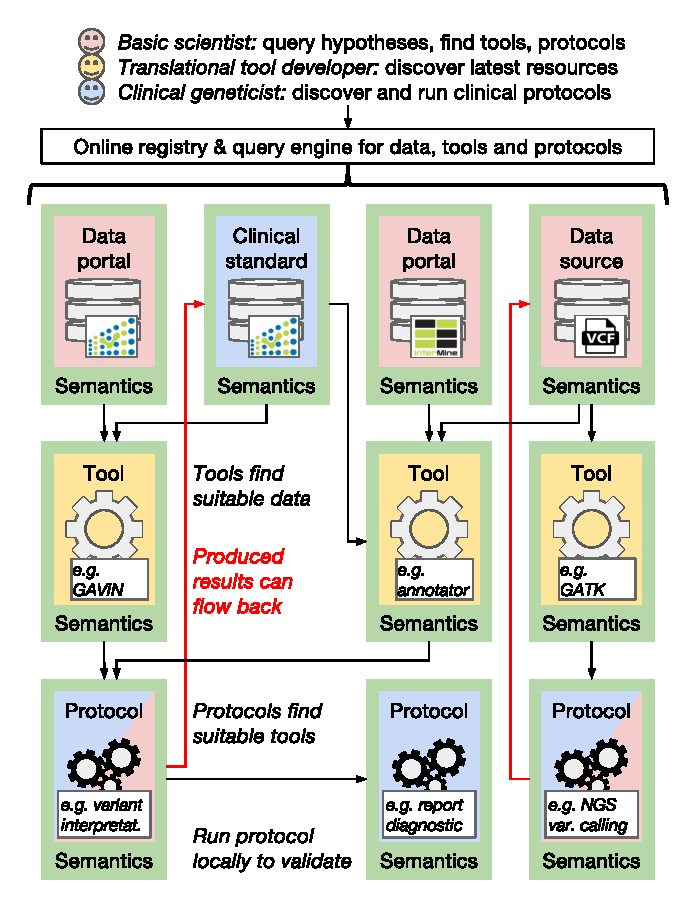
\includegraphics[scale=0.9]{img/discussion_futurevision}
\caption[Interplay between data, tools and protocols]{Overview of potential interplay between data, tools and protocols, all mediated by semantic definitions. The resources are self-descriptive and can be used in different scenarios by multiple disciplines in a synergistic knowledge feedback loop.}
\label{fig:discussion_futurevision}
\end{figure*}

Disconnecting tools and data from the protocols allows for designing and sharing of protocols without simultaneously dealing with implementation details, and prevents new protocols from having to be defined when a better tool that performs the same role is introduced.
When we extend this concept to tools that retrieve their own source data via semantic connection, the result is a moldable, future-proof workflow that ships with built-in validation and benchmarking.

The results created by tools or workflows may be automatically annotated with the appropriate semantics and can be fed back into knowledge repositories.
For example, after running a chain of tools that leads to variant classifications, an expert should be able to easily upload these results and share them with the community.
Such an approach helps us get the most value out of human experts, as their knowledge and decisions flow back into the system, catalyzing development of new and improved tools.

An immediate challenge to implement this concept is finding a place to keep the necessary tools, data and their metadata.
There are central repositories to help make patient mutations or sequencing reads meet FAIR principles, but there is no such place for the results of computational analyses.
While the model organism data in chapter \ref{chap:wormqtl} can be found through the major community hub \url{http://www.wormbase.org}, the data in chapter \ref{chap:gavin} is not so FAIR.
Both the article and data are free and open to the world, but the existence of the data set is not explicitly advertised or registered on a community hub, limiting its Findability.
Bioinformaticians and computational biologists must put more effort into placing their work in context with the original data, and we need take responsibility as a community to create new means of enabling this integration if there are no suitable solutions available.


\section{Conclusion}

Each topic in this thesis is part of the same mission: to let patients with genetic disorders benefit more from rapidly increasing biological data production and new knowledge.
More specifically, we want to obtain predictors and biomarkers from research and patient data that can quickly establish the best and earliest diagnosis or prognosis.
To achieve this goal, we integrated and make available big reference data in chapters \ref{chap:xgap} and \ref{chap:xqtl}, bridged model organism to human data in chapter \ref{chap:wormqtl}, translated generic methods into clinical applications in chapters \ref{chap:caddmmr} and \ref{chap:gavin}, and developed a platform to bring innovations into practice in chapter \ref{chap:frameworkforgenomics}.

The resources currently available are already plentiful, and both the amount and types of molecular life science data is growing at a tremendous pace.
This present us with incredible opportunities to develop new and exciting methods that are more powerful and better tailored to patients than ever before, but simultaneously introduces the huge challenge of integrating and understanding these data.
To keep up, we must work smarter by investing in development and implementation of techniques that bring data together and stimulate collaboration such as FAIR principles, sharing platforms and semantic web.
Our research, development and hands-on experience of MOLGENIS flexible databases with ontology annotation tools are ready to play a significant role here.

New molecular data modalities such as non-coding DNA, RNA expression and metabolic profiles are emerging, and corresponding tools for clinical application will continuously improve as the quantity and quality of gold standard data increases over time.
To keep complex multi-omics data pipelines manageable in practice, we need modular best practice workflows that have self-managing and self-validating properties.
With many methods available, and their strengths and limitations characterized, the most appropriate tools could be automatically selected to diagnose a patient with an individualized multi-biomarker approach.
The genomics platform that we are developing in combination with the MOLGENIS Compute engine is being used in a diagnostic setting already and should provide the flexibility to scale up and expand to future technologies.

In the future, I envision a seamless international collaboration of experts in an online community-based decision support system where research data, gold standards, tools, workflows, benchmarks and best practices may be shared freely and openly.
This will increase the effectiveness of clinical molecular diagnostics at a maximum speed and unlock the potential of all measurable omics data types.
We can further integrate these results with findings that may currently be difficult to interpret such as risk factors from genome wide association studies, effects in quantitative trait loci or allele-specific expression, changes in the microbiome, epigenetic marks, or multigenic inheritance.
Automatically generated reports will then present prioritized findings and other relevant insights along with any known limitations and uncertainties, so researchers and doctors have clear and honest understanding of the results.
Taken together, we will be able to translate the knowledge gained from research data, expert communities and computational methods into medical practice for fast, accurate and personalized patient care.
